% Table 1  -  Reporting-Delay Atlas. Generated by analysis/07_tables.py.
% Requires tables_preamble.tex.
\begin{table}[!ht]
\caption{Reporting-Delay Atlas: complaint counts, delay quantiles and reported-by
horizons for consumer-channel complaints, mature incident cohorts only
($t \leq$ 2023-06 $= T - D$). Shaded bars show the share reported within
1, 6 and 12 months; the right-hand sparkline traces the full delay CDF $F(d)$, $d = 0$--36 months.}
\label{tab:atlas}
\footnotesize
\centering
\begin{tabular}{@{}l r r r r r r l l l l@{}}
\toprule
 & & & \multicolumn{4}{c}{Delay (days)} & \multicolumn{3}{c}{Reported within}  & \multicolumn{1}{c}{\footnotesize Delay spread}\\
\cmidrule(lr){4-7}\cmidrule(lr){8-10}
Group & $N$ & \% & P25 & P50 & P75 & P90 & 1 mo & 6 mo & 12 mo  & \multicolumn{1}{c}{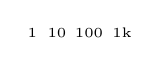
\begin{tikzpicture}[x=13mm,y=1mm,baseline=0mm]\node[anchor=base,inner sep=0pt,font=\tiny] at (0.098,0) {1};\node[anchor=base,inner sep=0pt,font=\tiny] at (0.338,0) {10};\node[anchor=base,inner sep=0pt,font=\tiny] at (0.651,0) {100};\node[anchor=base,inner sep=0pt,font=\tiny] at (0.974,0) {1k};\end{tikzpicture}}\\
\midrule
\textbf{All consumer complaints} & 1\,267\,531 & 100.0 & 3 & 20 & 136 & 480 & \dbar{0.640}{64} & \dbar{0.824}{82} & \dbar{0.905}{91} & \begin{tikzpicture}[x=13mm,y=1mm,baseline=-0.75mm]\draw[glyphgrid] (0.098,-1.25) -- (0.098,1.25);\draw[glyphgrid] (0.338,-1.25) -- (0.338,1.25);\draw[glyphgrid] (0.651,-1.25) -- (0.651,1.25);\draw[glyphgrid] (0.974,-1.25) -- (0.974,1.25);\draw[glyphaxis] (0,0) -- (1,0);\draw[whisker] (0.694,0) -- (0.871,0);\draw[whisker] (0.871,-0.62) -- (0.871,0.62);\fill[barfill] (0.196,-0.95) rectangle (0.694,0.95);\draw[medtick] (0.429,-1.25) -- (0.429,1.25);\end{tikzpicture} \\
\addlinespace[2pt]
\multicolumn{11}{@{}l}{\textit{By severity class}}\\
\hspace{0.8em}No injury (Y0) & 1\,142\,025 & 90.1 & 2 & 20 & 144 & 494 & \dbar{0.635}{64} & \dbar{0.819}{82} & \dbar{0.902}{90} & \begin{tikzpicture}[x=13mm,y=1mm,baseline=-0.75mm]\draw[glyphgrid] (0.098,-1.25) -- (0.098,1.25);\draw[glyphgrid] (0.338,-1.25) -- (0.338,1.25);\draw[glyphgrid] (0.651,-1.25) -- (0.651,1.25);\draw[glyphgrid] (0.974,-1.25) -- (0.974,1.25);\draw[glyphaxis] (0,0) -- (1,0);\draw[whisker] (0.702,0) -- (0.875,0);\draw[whisker] (0.875,-0.62) -- (0.875,0.62);\fill[barfill] (0.155,-0.95) rectangle (0.702,0.95);\draw[medtick] (0.429,-1.25) -- (0.429,1.25);\end{tikzpicture} \\
\hspace{0.8em}Crash/fire (Y1) & 71\,400 & 5.6 & 3 & 15 & 69 & 343 & \dbar{0.706}{71} & \dbar{0.878}{88} & \dbar{0.936}{94} & \begin{tikzpicture}[x=13mm,y=1mm,baseline=-0.75mm]\draw[glyphgrid] (0.098,-1.25) -- (0.098,1.25);\draw[glyphgrid] (0.338,-1.25) -- (0.338,1.25);\draw[glyphgrid] (0.651,-1.25) -- (0.651,1.25);\draw[glyphgrid] (0.974,-1.25) -- (0.974,1.25);\draw[glyphaxis] (0,0) -- (1,0);\draw[whisker] (0.599,0) -- (0.824,0);\draw[whisker] (0.824,-0.62) -- (0.824,0.62);\fill[barfill] (0.196,-0.95) rectangle (0.599,0.95);\draw[medtick] (0.391,-1.25) -- (0.391,1.25);\end{tikzpicture} \\
\hspace{0.8em}Injury (Y2) & 51\,920 & 4.1 & 4 & 19 & 88 & 380 & \dbar{0.670}{67} & \dbar{0.862}{86} & \dbar{0.925}{93} & \begin{tikzpicture}[x=13mm,y=1mm,baseline=-0.75mm]\draw[glyphgrid] (0.098,-1.25) -- (0.098,1.25);\draw[glyphgrid] (0.338,-1.25) -- (0.338,1.25);\draw[glyphgrid] (0.651,-1.25) -- (0.651,1.25);\draw[glyphgrid] (0.974,-1.25) -- (0.974,1.25);\draw[glyphaxis] (0,0) -- (1,0);\draw[whisker] (0.633,0) -- (0.838,0);\draw[whisker] (0.838,-0.62) -- (0.838,0.62);\fill[barfill] (0.227,-0.95) rectangle (0.633,0.95);\draw[medtick] (0.422,-1.25) -- (0.422,1.25);\end{tikzpicture} \\
\hspace{0.8em}Fatality (Y3) & 2\,186 & 0.2 & 21 & 99 & 465 & 1\,182 & \dbar{0.426}{43} & \dbar{0.675}{68} & \dbar{0.798}{80} & \begin{tikzpicture}[x=13mm,y=1mm,baseline=-0.75mm]\draw[glyphgrid] (0.098,-1.25) -- (0.098,1.25);\draw[glyphgrid] (0.338,-1.25) -- (0.338,1.25);\draw[glyphgrid] (0.651,-1.25) -- (0.651,1.25);\draw[glyphgrid] (0.974,-1.25) -- (0.974,1.25);\draw[glyphaxis] (0,0) -- (1,0);\draw[whisker] (0.866,0) -- (0.998,0);\draw[whisker] (0.998,-0.62) -- (0.998,0.62);\fill[barfill] (0.436,-0.95) rectangle (0.866,0.95);\draw[medtick] (0.649,-1.25) -- (0.649,1.25);\end{tikzpicture} \\
\addlinespace[2pt]
\multicolumn{11}{@{}l}{\textit{By reporting channel}}\\
\hspace{0.8em}Internet (IVOQ) & 845\,644 & 66.7 & 2 & 15 & 114 & 471 & \dbar{0.674}{67} & \dbar{0.837}{84} & \dbar{0.909}{91} & \begin{tikzpicture}[x=13mm,y=1mm,baseline=-0.75mm]\draw[glyphgrid] (0.098,-1.25) -- (0.098,1.25);\draw[glyphgrid] (0.338,-1.25) -- (0.338,1.25);\draw[glyphgrid] (0.651,-1.25) -- (0.651,1.25);\draw[glyphgrid] (0.974,-1.25) -- (0.974,1.25);\draw[glyphaxis] (0,0) -- (1,0);\draw[whisker] (0.669,0) -- (0.868,0);\draw[whisker] (0.868,-0.62) -- (0.868,0.62);\fill[barfill] (0.155,-0.95) rectangle (0.669,0.95);\draw[medtick] (0.391,-1.25) -- (0.391,1.25);\end{tikzpicture} \\
\hspace{0.8em}Hotline (EVOQ) & 396\,153 & 31.3 & 4 & 31 & 171 & 504 & \dbar{0.581}{58} & \dbar{0.802}{80} & \dbar{0.899}{90} & \begin{tikzpicture}[x=13mm,y=1mm,baseline=-0.75mm]\draw[glyphgrid] (0.098,-1.25) -- (0.098,1.25);\draw[glyphgrid] (0.338,-1.25) -- (0.338,1.25);\draw[glyphgrid] (0.651,-1.25) -- (0.651,1.25);\draw[glyphgrid] (0.974,-1.25) -- (0.974,1.25);\draw[glyphaxis] (0,0) -- (1,0);\draw[whisker] (0.726,0) -- (0.878,0);\draw[whisker] (0.878,-0.62) -- (0.878,0.62);\fill[barfill] (0.227,-0.95) rectangle (0.726,0.95);\draw[medtick] (0.489,-1.25) -- (0.489,1.25);\end{tikzpicture} \\
\hspace{0.8em}Questionnaire (VOQ) & 25\,534 & 2.0 & 14 & 62 & 221 & 450 & \dbar{0.448}{45} & \dbar{0.740}{74} & \dbar{0.875}{87} & \begin{tikzpicture}[x=13mm,y=1mm,baseline=-0.75mm]\draw[glyphgrid] (0.098,-1.25) -- (0.098,1.25);\draw[glyphgrid] (0.338,-1.25) -- (0.338,1.25);\draw[glyphgrid] (0.651,-1.25) -- (0.651,1.25);\draw[glyphgrid] (0.974,-1.25) -- (0.974,1.25);\draw[glyphaxis] (0,0) -- (1,0);\draw[whisker] (0.762,0) -- (0.862,0);\draw[whisker] (0.862,-0.62) -- (0.862,0.62);\fill[barfill] (0.382,-0.95) rectangle (0.762,0.95);\draw[medtick] (0.584,-1.25) -- (0.584,1.25);\end{tikzpicture} \\
\hspace{0.8em}Mobile app (MAVQ) & 200 & 0.0 & 0 & 8 & 92 & 391 & \dbar{0.708}{71} & \dbar{0.851}{85} & \dbar{0.923}{92} & \begin{tikzpicture}[x=13mm,y=1mm,baseline=-0.75mm]\draw[glyphgrid] (0.098,-1.25) -- (0.098,1.25);\draw[glyphgrid] (0.338,-1.25) -- (0.338,1.25);\draw[glyphgrid] (0.651,-1.25) -- (0.651,1.25);\draw[glyphgrid] (0.974,-1.25) -- (0.974,1.25);\draw[glyphaxis] (0,0) -- (1,0);\draw[whisker] (0.639,0) -- (0.842,0);\draw[whisker] (0.842,-0.62) -- (0.842,0.62);\fill[barfill] (0.000,-0.95) rectangle (0.639,0.95);\draw[medtick] (0.302,-1.25) -- (0.302,1.25);\end{tikzpicture} \\
\addlinespace[2pt]
\multicolumn{11}{@{}l}{\textit{By incident-cohort era}}\\
\hspace{0.8em}1995--2004 & 278\,467 & 22.0 & 5 & 31 & 166 & 522 & \dbar{0.589}{59} & \dbar{0.805}{80} & \dbar{0.895}{90} & \begin{tikzpicture}[x=13mm,y=1mm,baseline=-0.75mm]\draw[glyphgrid] (0.098,-1.25) -- (0.098,1.25);\draw[glyphgrid] (0.338,-1.25) -- (0.338,1.25);\draw[glyphgrid] (0.651,-1.25) -- (0.651,1.25);\draw[glyphgrid] (0.974,-1.25) -- (0.974,1.25);\draw[glyphaxis] (0,0) -- (1,0);\draw[whisker] (0.722,0) -- (0.883,0);\draw[whisker] (0.883,-0.62) -- (0.883,0.62);\fill[barfill] (0.253,-0.95) rectangle (0.722,0.95);\draw[medtick] (0.489,-1.25) -- (0.489,1.25);\end{tikzpicture} \\
\hspace{0.8em}2005--2014 & 460\,607 & 36.3 & 3 & 23 & 182 & 655 & \dbar{0.621}{62} & \dbar{0.801}{80} & \dbar{0.887}{89} & \begin{tikzpicture}[x=13mm,y=1mm,baseline=-0.75mm]\draw[glyphgrid] (0.098,-1.25) -- (0.098,1.25);\draw[glyphgrid] (0.338,-1.25) -- (0.338,1.25);\draw[glyphgrid] (0.651,-1.25) -- (0.651,1.25);\draw[glyphgrid] (0.974,-1.25) -- (0.974,1.25);\draw[glyphaxis] (0,0) -- (1,0);\draw[whisker] (0.735,0) -- (0.915,0);\draw[whisker] (0.915,-0.62) -- (0.915,0.62);\fill[barfill] (0.196,-0.95) rectangle (0.735,0.95);\draw[medtick] (0.448,-1.25) -- (0.448,1.25);\end{tikzpicture} \\
\hspace{0.8em}2015--2023 & 528\,457 & 41.7 & 2 & 13 & 93 & 367 & \dbar{0.683}{68} & \dbar{0.854}{85} & \dbar{0.926}{93} & \begin{tikzpicture}[x=13mm,y=1mm,baseline=-0.75mm]\draw[glyphgrid] (0.098,-1.25) -- (0.098,1.25);\draw[glyphgrid] (0.338,-1.25) -- (0.338,1.25);\draw[glyphgrid] (0.651,-1.25) -- (0.651,1.25);\draw[glyphgrid] (0.974,-1.25) -- (0.974,1.25);\draw[glyphaxis] (0,0) -- (1,0);\draw[whisker] (0.641,0) -- (0.833,0);\draw[whisker] (0.833,-0.62) -- (0.833,0.62);\fill[barfill] (0.155,-0.95) rectangle (0.641,0.95);\draw[medtick] (0.372,-1.25) -- (0.372,1.25);\end{tikzpicture} \\
\bottomrule
\end{tabular}
\end{table}
